\documentclass[tikz,border=2pt]{standalone}

\usepackage[sfdefault]{FiraSans}
\usepackage{FiraMono}
\usepackage{etoolbox}
\usepackage{xcolor}
\usetikzlibrary{arrows.meta,calc,matrix,shapes.geometric}

\providecommand{\diaglang}{pt}
\ifdefstring{\diaglang}{pt}{}{%
  \ifdefstring{\diaglang}{en}{}{%
    \PackageError{terravault-runtime-architecture-v5}{Unsupported language '\diaglang'}{Use pt or en.}%
  }%
}

\newcommand{\LText}[2]{\ifdefstring{\diaglang}{pt}{#1}{#2}}
\newcommand{\Literal}[1]{{\ttfamily #1}}
\newcommand{\PlateTitleFont}{\fontsize{21}{23}\selectfont\bfseries}
\newcommand{\PlateSubtitleFont}{\fontsize{11.5}{14}\selectfont\mdseries}
\newcommand{\TitleFont}{\fontsize{14.5}{16.5}\selectfont\mdseries}
\newcommand{\SubtitleFont}{\fontsize{10.8}{12.5}\selectfont\mdseries}
\newcommand{\EdgeFont}{\fontsize{9.8}{11.2}\selectfont\mdseries}
\newcommand{\GroupFont}{\fontsize{12.5}{14}\selectfont\bfseries}
\newcommand{\LegendFont}{\fontsize{9.5}{11}\selectfont\mdseries}
\newcommand{\FootnoteFont}{\fontsize{10.2}{11.9}\selectfont\mdseries}
\newcommand{\NodeText}[2]{{\TitleFont #1}\\[1.0mm]{\SubtitleFont #2}}

% Node labels wrap at spaces only, and every text width in this plate is sized
% from the measured width of its longest line in *both* languages. Multi-line
% labels break where they are written to break: automatic wrapping pushed
% separators such as "·" to the start of continuation lines in v2, which reads
% as a bullet list rather than a phrase.
\hyphenpenalty=10000
\exhyphenpenalty=10000

\definecolor{orchestration}{HTML}{16324F}
\definecolor{ruleDetection}{HTML}{2E5E7E}
\definecolor{mlPath}{HTML}{17786A}
\definecolor{scoreDecision}{HTML}{E9A13B}
\definecolor{infrastructure}{HTML}{4E5A66}
\definecolor{infrastructureTop}{HTML}{636E78}
\definecolor{mlPathTop}{HTML}{33887C}
\definecolor{groupBoundaryColour}{HTML}{8A97A3}
\definecolor{edgeColour}{HTML}{3C4650}
\definecolor{edgeLabelColour}{HTML}{56626E}
\definecolor{panelTint}{HTML}{F7F9FA}

\tikzset{
  base node/.style={
    draw=none,
    rounded corners=1.6mm,
    align=center,
    inner xsep=2.5mm,
    inner ysep=2.1mm,
    minimum height=1.28cm,
    text=white
  },
  io node/.style={base node,fill=infrastructure},
  orchestration node/.style={base node,fill=orchestration},
  rule node/.style={base node,fill=ruleDetection},
  ml node/.style={base node,fill=mlPath},
  score node/.style={base node,fill=scoreDecision,text=orchestration},
  % Outlined boxes are files on a volume, not processes. The convention covers
  % every mounted or written artifact and nothing else.
  artifact node/.style={
    draw=infrastructure,
    line width=0.9pt,
    rounded corners=1.6mm,
    fill=white,
    text=orchestration,
    align=center,
    inner xsep=2.4mm,
    inner ysep=1.9mm,
    minimum height=1.25cm
  },
  model artifact/.style={
    artifact node,
    draw=mlPath,
    text=mlPath,
    line width=1.2pt
  },
  storage node/.style={
    shape=cylinder,
    shape border rotate=90,
    aspect=0.11,
    cylinder uses custom fill,
    cylinder body fill=infrastructure,
    cylinder end fill=infrastructureTop,
    draw=none,
    align=center,
    inner xsep=2.5mm,
    inner ysep=1.7mm,
    minimum height=1.38cm,
    text=white
  },
  panel/.style={
    draw=groupBoundaryColour,
    line width=0.65pt,
    rounded corners=1.8mm,
    fill=panelTint
  },
  deployment boundary/.style={
    draw=groupBoundaryColour,
    dashed,
    dash pattern=on 3.2mm off 1.8mm,
    line width=0.85pt,
    rounded corners=1.8mm
  },
  panel label/.style={
    anchor=north west,
    font=\GroupFont,
    text=orchestration,
    fill=panelTint,
    inner xsep=1.2mm,
    inner ysep=0.7mm
  },
  edge base/.style={draw=edgeColour,line width=1.05pt,line cap=round,line join=round},
  flow/.style={edge base,-{Stealth[length=2.35mm,width=1.55mm]}},
  pull/.style={flow,dashed,dash pattern=on 2.4mm off 1.7mm},
  mount/.style={flow,dotted,dash pattern=on 0.35mm off 1.25mm,line width=1.25pt},
  % Dash-dot is reserved for the PostgreSQL write: the API logs persistence
  % failure but still returns a successful scan. Redis stays a solid runtime
  % call because Compose health-gates startup and the normal limiter uses it.
  best effort/.style={flow,dash pattern=on 3.2mm off 1.4mm on 0.45mm off 1.4mm},
  % A branch is drawn once as a trunk plus arrowed legs, with the junction
  % marked. v2 drew each leg as a full path, overprinting the shared segment.
  junction/.style={circle,fill=edgeColour,inner sep=0pt,minimum size=1.55mm},
  % Every edge label is declared inline on the path it belongs to, so it is
  % centred *in* the line rather than floating beside it: the fill matches the
  % panel, and the label reads as a gap in the edge it names. Up to v4 these
  % were free-standing nodes placed above the line at hand-measured
  % coordinates, which left long runs whose label could equally have belonged
  % to the row above. Because the label now occupies the line, every lane in
  % this plate is sized to hold its own longest string in either language,
  % measured, plus clearance at both ends.
  edge label/.style={
    font=\EdgeFont,
    text=edgeLabelColour,
    fill=panelTint,
    inner xsep=1.0mm,
    inner ysep=0.6mm,
    align=center
  },
  % Annotations carry the semantics a line style can only hint at. They are the
  % only text that is deliberately *not* on an edge; each one sits next to the
  % single node it qualifies.
  annotation/.style={
    font=\FootnoteFont,
    text=edgeLabelColour,
    fill=panelTint,
    inner xsep=1.0mm,
    inner ysep=0.5mm,
    align=center
  },
  legend swatch/.style={minimum width=3.2mm,minimum height=3.2mm,inner sep=0pt,draw=none},
  % The outlined-box convention was documented in the source and drawn on the
  % plate, but never keyed: a reader saw a sixth treatment with no entry
  % explaining it. The swatch is drawn grey because outline colour still
  % carries the category (grey infrastructure, teal ML) — outline *versus*
  % fill is the only thing this entry names.
  legend artifact swatch/.style={
    minimum width=3.2mm,
    minimum height=3.2mm,
    inner sep=0pt,
    draw=infrastructure,
    line width=0.9pt,
    rounded corners=0.55mm,
    fill=white
  },
  legend line/.style={minimum width=9mm,minimum height=3.2mm,inner sep=0pt},
  legend solid/.style={
    legend line,
    path picture={
      \draw[edge base]
        ([xshift=0.5mm]path picture bounding box.west) --
        ([xshift=-0.5mm]path picture bounding box.east);
    }
  },
  legend dashed/.style={
    legend line,
    path picture={
      \draw[edge base,dashed,dash pattern=on 2.4mm off 1.7mm]
        ([xshift=0.5mm]path picture bounding box.west) --
        ([xshift=-0.5mm]path picture bounding box.east);
    }
  },
  legend dotted/.style={
    legend line,
    path picture={
      \draw[edge base,dotted,dash pattern=on 0.35mm off 1.25mm,line width=1.25pt]
        ([xshift=0.5mm]path picture bounding box.west) --
        ([xshift=-0.5mm]path picture bounding box.east);
    }
  },
  legend dashdotted/.style={
    legend line,
    path picture={
      \draw[edge base,dash pattern=on 3.2mm off 1.4mm on 0.45mm off 1.4mm]
        ([xshift=0.5mm]path picture bounding box.west) --
        ([xshift=-0.5mm]path picture bounding box.east);
    }
  }
}

\begin{document}
% This plate deliberately separates deployment topology from the logical scan
% pipeline. The latter is drawn once, even though the same Python package runs
% in either the terravault-api container or the local CLI process.
%
% Every figure on it is checked against the tree: 11 rules in
% domain/security_rules.py; an 8-column vector in
% application/feature_extraction.py; int(0.6·rules + 0.4·ml) in
% application/scanner.py; the scan/vulnerability persistence path; the two :ro
% mounts, the 10 MB cap and the 30 s timeout in docker-compose.yml; the route
% allowlist and the private-range /metrics handler in Caddyfile; the normal
% 10/minute /scan limit and configured 100/minute process fallback in api.py;
% the job-level 10s scrape in monitoring/prometheus.yml.
%
% Horizontal space is the scarce axis: the plate is rasterised at a fixed
% width, so a wider canvas shrinks every glyph, while extra height is free.
% Rows are therefore spread vertically and columns are packed only as far as
% the edge label between them allows.
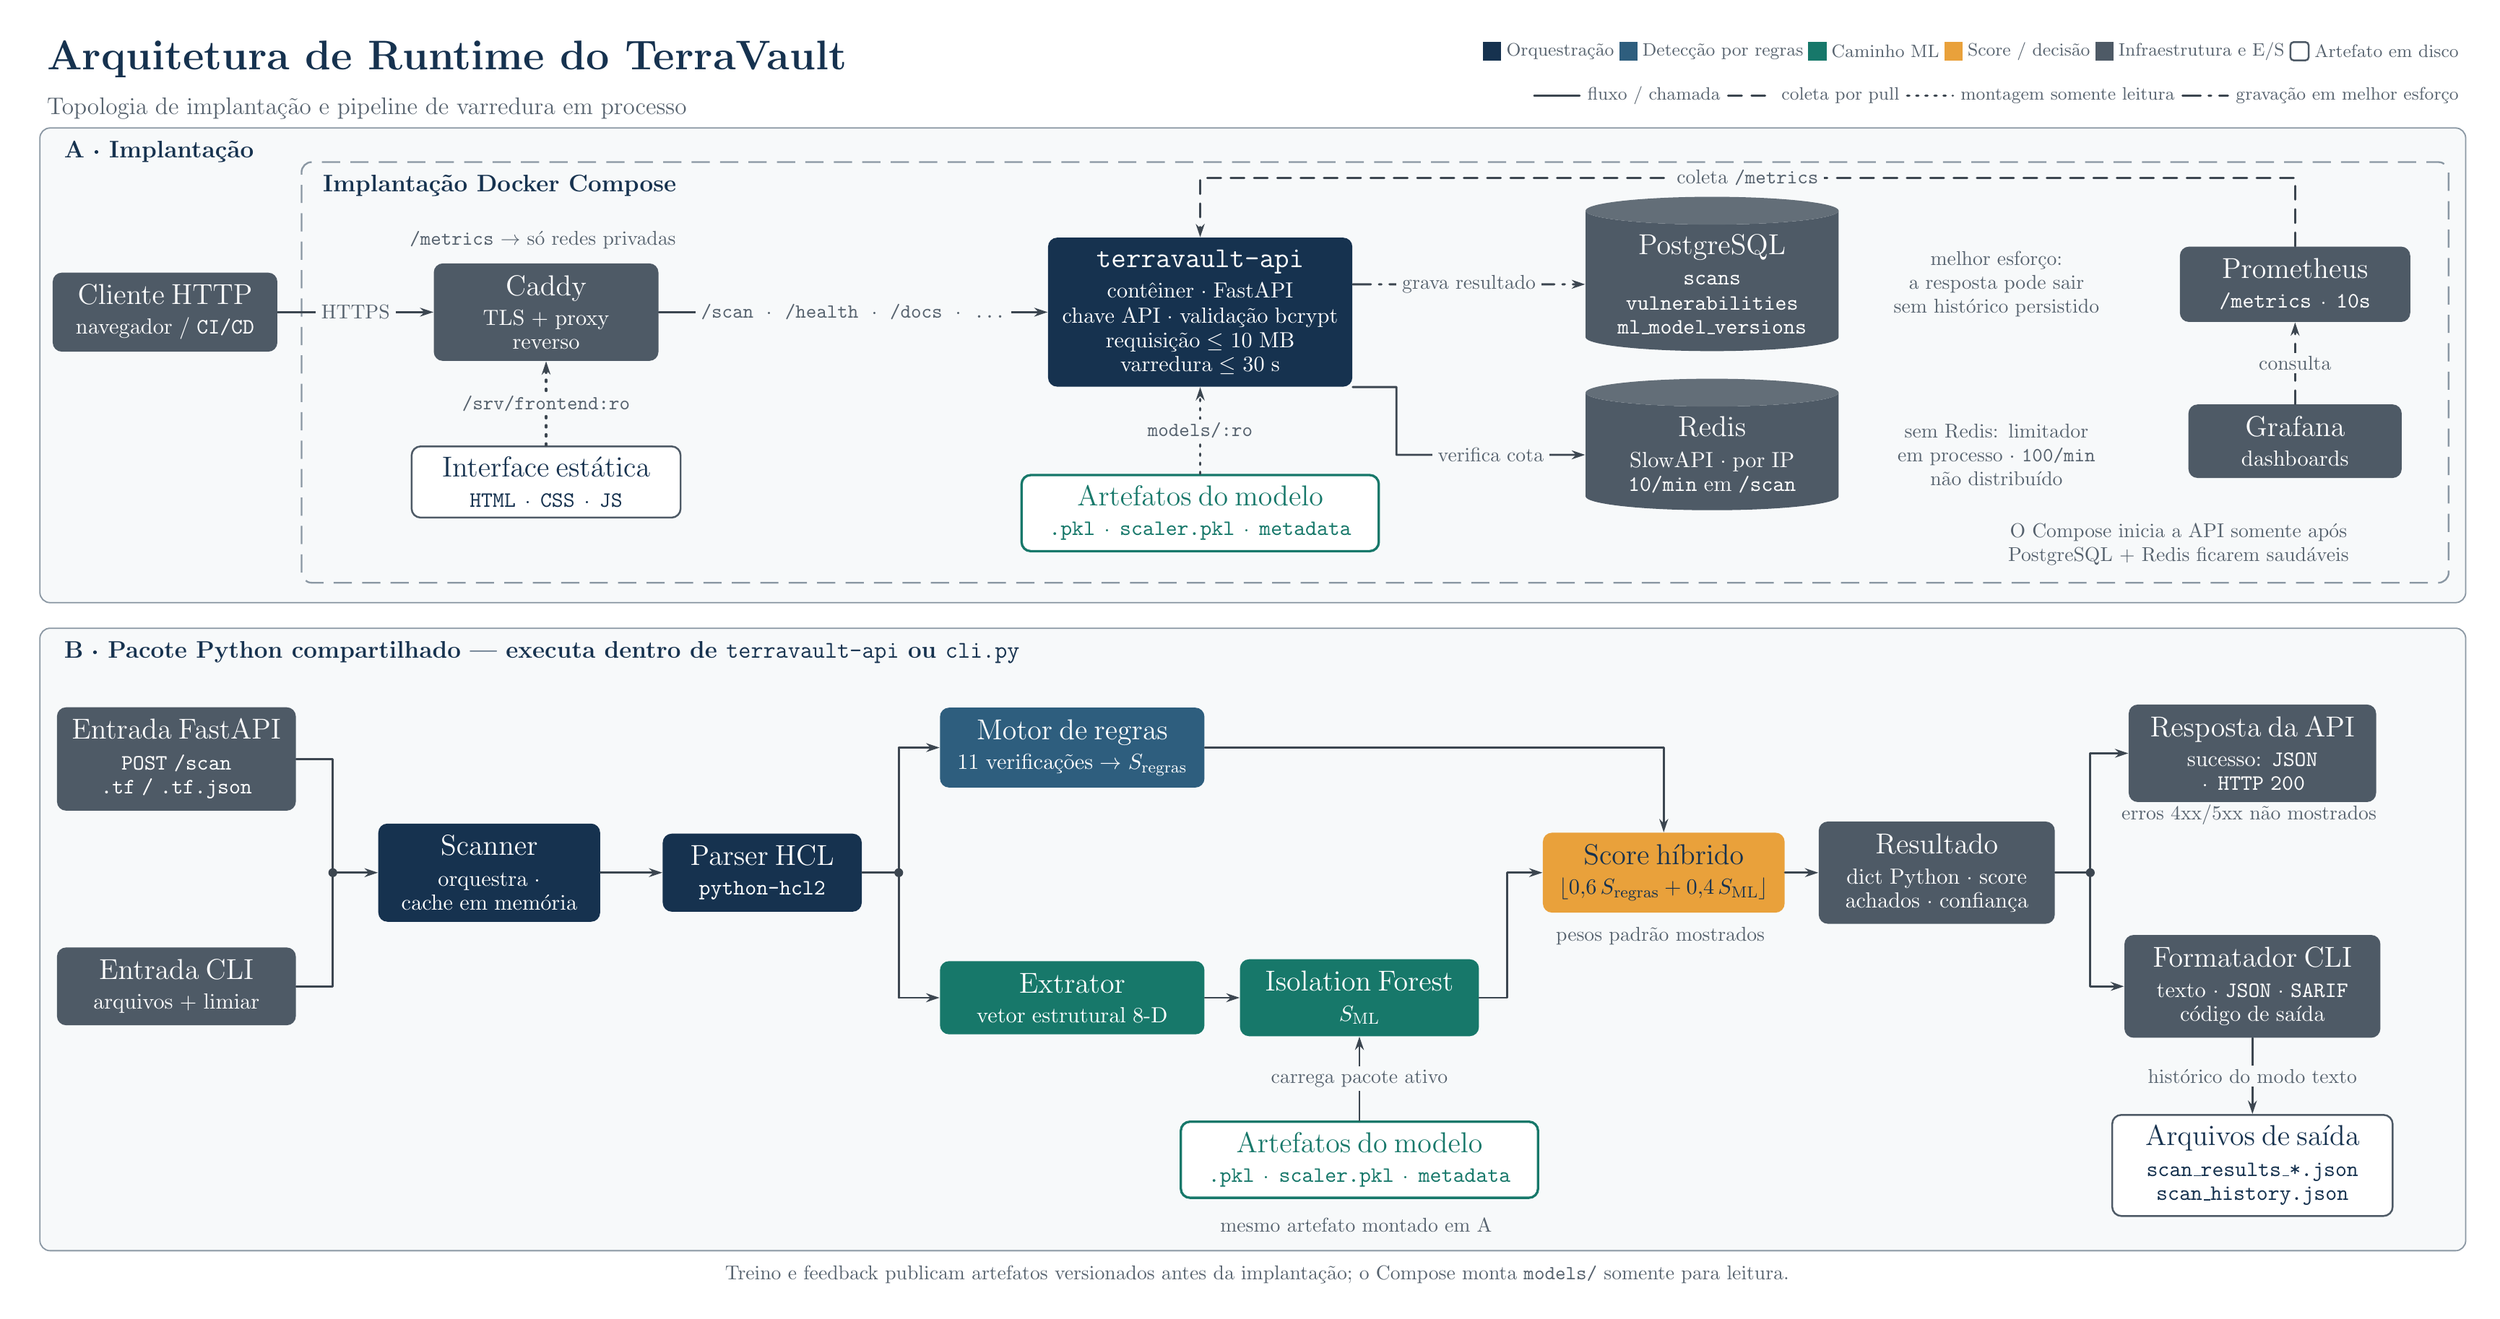
\begin{tikzpicture}[x=0.5cm,y=0.5cm]
  \path[use as bounding box] (-0.5,-3.3) rectangle (86.0,41.7);
  \fill[white] (-0.5,-3.3) rectangle (86.0,41.7);

  \node[font=\PlateTitleFont,text=orchestration,anchor=north west] at (0.2,41.2) {
    \LText{Arquitetura de Runtime do TerraVault}{TerraVault Runtime Architecture}
  };
  \node[font=\PlateSubtitleFont,text=edgeLabelColour,anchor=north west] at (0.2,39.2) {
    \LText{Topologia de implantação e pipeline de varredura em processo}
      {Deployment topology and in-process scan pipeline}
  };

  % Two matrices, not one: a single matrix shares column widths across rows, so
  % the colour row and the line-style row could not both sit flush right.
  \matrix[
    matrix of nodes,
    anchor=north east,
    column sep=0.9mm,
    nodes={font=\LegendFont,text=edgeLabelColour,anchor=west,inner sep=0pt}
  ] at (85.5,41.2) {
    |[legend swatch,fill=orchestration]| {} & \LText{Orquestração}{Orchestration} &
    |[legend swatch,fill=ruleDetection]| {} & \LText{Detecção por regras}{Rule detection} &
    |[legend swatch,fill=mlPath]| {} & \LText{Caminho ML}{ML path} &
    |[legend swatch,fill=scoreDecision]| {} & \LText{Score / decisão}{Score / decision} &
    |[legend swatch,fill=infrastructure]| {} & \LText{Infraestrutura e E/S}{Infrastructure and I/O} &
    |[legend artifact swatch]| {} & \LText{Artefato em disco}{Artifact on disk} \\
  };

  \matrix[
    matrix of nodes,
    anchor=north east,
    column sep=0.9mm,
    nodes={font=\LegendFont,text=edgeLabelColour,anchor=west,inner sep=0pt}
  ] at (85.5,39.6) {
    |[legend solid]| {} & \LText{fluxo / chamada}{flow / call} &
    |[legend dashed]| {} & \LText{coleta por pull}{pull collection} &
    |[legend dotted]| {} & \LText{montagem somente leitura}{read-only mount} &
    |[legend dashdotted]| {} & \LText{gravação em melhor esforço}{best-effort write} \\
  };

  % ------------------------------------------------------------------------
  % Panel A: concrete Docker Compose topology. Only real services and mounted
  % artifacts appear here; the static UI is not presented as a container.
  % ------------------------------------------------------------------------
  % The panel label is opaque, so it must end before the Compose boundary's
  % top-left corner or it knocks a gap out of the dashed edge. That caps the
  % label at roughly 9 units in both languages.
  \draw[panel] (0.2,21.2) rectangle (85.5,37.9);
  \node[panel label] at (0.8,37.6) {
    \LText{A · Implantação}{A · Deployment view}
  };
  % The boundary starts at 9.4 so the HTTPS label, centred in the client edge,
  % clears the dashed rule instead of appearing to cut it.
  \draw[deployment boundary] (9.4,21.9) rectangle (84.9,36.7);
  \node[panel label] at (9.9,36.4) {
    \LText{Implantação Docker Compose}{Docker Compose deployment}
  };

  \node[io node,text width=3.45cm] (client) at (4.6,31.42) {
    \NodeText{\LText{Cliente HTTP}{HTTP client}}
      {\LText{navegador / \Literal{CI/CD}}{browser / \Literal{CI/CD}}}
  };
  \node[artifact node,text width=4.25cm] (staticui) at (18.0,25.445) {
    \NodeText{\LText{Interface estática}{Static web UI}}
      {\Literal{HTML · CSS · JS}}
  };
  \node[io node,text width=3.45cm] (caddy) at (18.0,31.42) {
    \NodeText{Caddy}
      {\LText{TLS + proxy reverso}{TLS + reverse proxy}}
  };
  \node[orchestration node,text width=4.85cm] (api) at (41.0,31.42) {
    \NodeText{\Literal{terravault-api}}
      {\LText{contêiner}{container} · FastAPI\\
       \LText{chave API · validação bcrypt}{API key · bcrypt-verified}\\
       \LText{requisição $\leq$ 10 MB}{request $\leq$ 10 MB}\\
       \LText{varredura $\leq$ 30 s}{scan $\leq$ 30 s}}
  };
  \node[model artifact,text width=5.8cm] (runtimeModel) at (41.0,24.35) {
    \NodeText{\LText{Artefatos do modelo}{Model artifacts}}
      {\Literal{.pkl · scaler.pkl · metadata}}
  };
  % All three tables, not the two on the scan path: ml_model_versions is a real
  % table in infrastructure/models.py, and listing only what the labelled write
  % edge touches made the store look smaller than it is. Provenance is already
  % carried by the plate footnote — the training run writes the version row,
  % the scan does not.
  \node[storage node,text width=3.95cm] (postgres) at (59.0,32.4) {
    \NodeText{PostgreSQL}
      {\Literal{scans}\\\Literal{vulnerabilities}\\\Literal{ml\_model\_versions}}
  };
  \node[storage node,text width=3.95cm] (redis) at (59.0,26.4) {
    \NodeText{Redis}
      {\LText{SlowAPI · por IP}{SlowAPI · per-IP}\\
       \Literal{10/min} \LText{em}{on} \Literal{/scan}}
  };
  \node[io node,text width=3.55cm] (prometheus) at (79.5,32.4) {
    \NodeText{Prometheus}{\Literal{/metrics · 10s}}
  };
  \node[io node,text width=3.25cm] (grafana) at (79.5,26.88) {
    \NodeText{Grafana}{dashboards}
  };

  \draw[flow] (client.east) -- node[edge label] {HTTPS} (caddy.west);

  \draw[mount] (staticui.north) --
    node[edge label] {\Literal{/srv/frontend:ro}} (caddy.south);

  % The proxy publishes an explicit allowlist, so the routes belong on the edge.
  \draw[flow] (caddy.east) --
    node[edge label] {\Literal{/scan · /health · /docs · \ldots}} (api.west);

  % /metrics answers only inside private ranges, which is what lets the
  % in-network scrape below succeed while the public path returns 404.
  \node[annotation,anchor=south] (metricsNote) at (18.0,33.53) {
    \Literal{/metrics} $\to$ \LText{só redes privadas}{private ranges only}
  };

  \draw[mount] (runtimeModel.north) --
    node[edge label] {\Literal{models/:ro}} (api.south);

  % Each store keeps its qualifier directly underneath it. Up to v4 both notes
  % sat in a column to the right of the cylinders, which is exactly the band
  % the write and quota edges now need in order to carry their own labels.
  \draw[best effort] (api.east |- postgres) --
    node[edge label] {\LText{grava resultado}{stores result}} (postgres.west);
  \node[annotation,text width=4.55cm] (pgNote) at (69.0,32.4) {
    \LText{melhor esforço:\\a resposta pode sair\\sem histórico persistido}
      {best effort:\\response may succeed\\without stored history}
  };

  \draw[flow] (api.south east) -- (47.9,0 |- api.south) -- (47.9,26.4) --
    node[edge label] {\LText{verifica cota}{checks quota}} (redis.west);
  \node[annotation,text width=4.55cm] (redisNote) at (69.0,26.4) {
    \LText{sem Redis: limitador\\em processo · \Literal{100/min}\\não distribuído}
      {without Redis:\\in-process limiter\\\Literal{100/min} · not distributed}
  };
  \node[annotation,text width=7.2cm] (composeNote) at (75.4,23.25) {
    \LText{O Compose inicia a API somente após PostgreSQL + Redis ficarem saudáveis}
      {Compose starts the API only after PostgreSQL + Redis are healthy}
  };

  % Prometheus initiates the scrape request, so the arrow points to the API.
  % The run sits at 36.15, not 35.8: the third table in the PostgreSQL cylinder
  % grew it upwards, and its own label is centred at x = 60.25 — directly over
  % that cylinder. 36.15 keeps clearance on both sides of the run without
  % touching the Compose boundary at 36.7.
  \draw[pull] (prometheus.north) -- (79.5,36.15) --
    node[edge label] {\LText{coleta \Literal{/metrics}}{scrapes \Literal{/metrics}}}
    (41.0,36.15) -- (api.north);

  % Stacking Grafana under Prometheus turns the query into a vertical edge,
  % which costs no horizontal space and still carries its own label.
  \draw[pull] (grafana.north) --
    node[edge label] {\LText{consulta}{queries}} (prometheus.south);

  % ------------------------------------------------------------------------
  % Panel B: one logical rendering of the shared package. Output adapters sit at
  % the far right so no return arrow has to travel back across the plate.
  % ------------------------------------------------------------------------
  \draw[panel] (0.2,-1.6) rectangle (85.5,20.3);
  \node[panel label] at (0.8,20.0) {
    \LText{B · Pacote Python compartilhado — executa dentro de \Literal{terravault-api} ou \Literal{cli.py}}
      {B · Shared Python package — runs inside \Literal{terravault-api} or \Literal{cli.py}}
  };

  \node[io node,text width=3.7cm] (apiInput) at (5.0,15.7) {
    \NodeText{\LText{Entrada FastAPI}{FastAPI input}}
      {\Literal{POST /scan}\\\Literal{.tf / .tf.json}}
  };
  \node[io node,text width=3.7cm] (cliInput) at (5.0,7.7) {
    \NodeText{\LText{Entrada CLI}{CLI input}}
      {\LText{arquivos + limiar}{files + threshold}}
  };
  \node[orchestration node,text width=3.4cm] (scanner) at (16.0,11.7) {
    \NodeText{Scanner}
      {\LText{orquestra ·\\cache em memória}{orchestrates ·\\memory cache}}
  };
  \node[orchestration node,text width=3.0cm] (parser) at (25.6,11.7) {
    \NodeText{\LText{Parser HCL}{HCL parser}}{\Literal{python-hcl2}}
  };
  \node[rule node,text width=4.15cm] (rules) at (36.5,16.1) {
    \NodeText{\LText{Motor de regras}{Rule engine}}
      {\LText{11 verificações $\to S_{\mathrm{regras}}$}{11 checks $\to S_{\mathrm{rules}}$}}
  };
  \node[ml node,text width=4.15cm] (extractor) at (36.5,7.3) {
    \NodeText{\LText{Extrator}{Extractor}}
      {\LText{vetor estrutural 8-D}{8-D structural vector}}
  };
  \node[ml node,text width=3.7cm] (isolation) at (46.6,7.3) {
    \NodeText{Isolation Forest}{$S_{\mathrm{ML}}$}
  };
  \node[score node,text width=3.75cm] (score) at (57.3,11.7) {
    \NodeText{\LText{Score híbrido}{Hybrid score}}
      {\LText{$\lfloor 0{,}6\,S_{\mathrm{regras}} + 0{,}4\,S_{\mathrm{ML}} \rfloor$}
        {$\lfloor 0.6\,S_{\mathrm{rules}} + 0.4\,S_{\mathrm{ML}} \rfloor$}}
  };
  \node[io node,text width=3.65cm] (result) at (66.9,11.7) {
    \NodeText{\LText{Resultado}{Scan result}}
      {\LText{dict Python · score\\achados · confiança}{Python dict · score\\findings · confidence}}
  };
  \node[io node,text width=3.85cm] (apiOutput) at (78.0,15.9) {
    \NodeText{\LText{Resposta da API}{API response}}
      {\LText{sucesso:}{success:} \Literal{JSON · HTTP 200}}
  };
  \node[io node,text width=4.0cm] (cliOutput) at (78.0,7.7) {
    \NodeText{\LText{Formatador CLI}{CLI formatter}}
      {\LText{texto · \Literal{JSON} · \Literal{SARIF}}{text · \Literal{JSON} · \Literal{SARIF}}\\
       \LText{código de saída}{exit code}}
  };
  \node[artifact node,text width=4.45cm] (outputFiles) at (78.0,1.4) {
    \NodeText{\LText{Arquivos de saída}{Output files}}
      {\Literal{scan\_results\_*.json}\\\Literal{scan\_history.json}}
  };
  % Same name and same contents as panel A: one artifact, drawn in two views.
  \node[model artifact,text width=5.8cm] (model) at (46.6,1.6) {
    \NodeText{\LText{Artefatos do modelo}{Model artifacts}}
      {\Literal{.pkl · scaler.pkl · metadata}}
  };

  \draw[edge base] (apiInput.east) -- (10.5,15.7) -- (10.5,11.7);
  \draw[edge base] (cliInput.east) -- (10.5,7.7) -- (10.5,11.7);
  \draw[flow] (10.5,11.7) -- (scanner.west);
  \node[junction] at (10.5,11.7) {};

  \draw[flow] (scanner.east) -- (parser.west);

  \draw[edge base] (parser.east) -- (30.4,11.7);
  \draw[edge base] (30.4,16.1) -- (30.4,7.3);
  \draw[flow] (30.4,16.1) -- (rules.west);
  \draw[flow] (30.4,7.3) -- (extractor.west);
  \node[junction] at (30.4,11.7) {};

  \draw[flow] (rules.east) -| (score.north);

  \draw[flow] (extractor.east) -- (isolation.west);
  \draw[edge base] (isolation.east) -- (51.8,7.3) -- (51.8,11.7);
  \draw[flow] (51.8,11.7) -- (score.west);

  \draw[flow] (score.east) -- (result.west);
  \node[annotation,anchor=north] (weightsNote) at (57.3,9.9) {
    \LText{pesos padrão mostrados}{default weights shown}
  };

  \draw[edge base] (result.east) -- (72.3,11.7);
  \draw[edge base] (72.3,15.9) -- (72.3,7.7);
  \draw[flow] (72.3,15.9) -- (apiOutput.west);
  \draw[flow] (72.3,7.7) -- (cliOutput.west);
  \node[junction] at (72.3,11.7) {};

  \draw[flow] (cliOutput.south) --
    node[edge label] {\LText{histórico do modo texto}{text-mode history}} (outputFiles.north);

  \draw[flow] (model.north) --
    node[edge label] {\LText{carrega pacote ativo}{loads active bundle}} (isolation.south);
  \node[annotation,anchor=north] (sameArtifactNote) at (46.6,-0.35) {
    \LText{mesmo artefato montado em A}{same artifact mounted in A}
  };
  \node[annotation,anchor=north] (errorsNote) at (78.0,14.2) {
    \LText{erros 4xx/5xx não mostrados}{4xx/5xx errors not shown}
  };

  \node[font=\FootnoteFont,text=edgeLabelColour,anchor=south] at (43.0,-3.0) {
    \LText{Treino e feedback publicam artefatos versionados antes da implantação; o Compose monta \Literal{models/} somente para leitura.}
      {Training and feedback publish versioned artifacts before deployment; Compose mounts \Literal{models/} read-only.}
  };
\end{tikzpicture}
\end{document}
